\documentclass[doc,floatsintext]{apa6}

\usepackage[english]{babel}
\usepackage[utf8x]{inputenc}
\usepackage[natbibapa]{apacite}%For APA referencing
\usepackage{amsfonts}
\usepackage{amsmath}
\usepackage{graphicx}
\usepackage{authblk}
\usepackage{microtype}
\usepackage{amssymb}
\usepackage{soul}
\usepackage[prependcaption,colorinlistoftodos]{todonotes}
\usepackage{amsmath}
\usepackage{algorithm}
\usepackage{algpseudocode}
\graphicspath{{Figures/}}

%For possessive citing
% \def\citeapos#1{\citeauthor{#1}'s (\citeyear{#1})}

% %to do notes jp
% \definecolor{aliceblue}{rgb}{0.94, 0.97, 1.0}
% \newcommand{\jptodo}[2][]{\todo[caption={\textbf{NB}}, size=\scriptsize, color = aliceblue, #1]{#2}~}
% \newcommand{\jptodo}[2][]{\vspace{0.1cm} \hfil \todo[caption={\textbf{JP}}, size=\footnotesize, color = aliceblue, inline, #1]{#2}}


\title{\textbf{Cascades across networks are sufficient for the formation of echo chambers: An agent-based model}}

\shorttitle{Network Cascades and Echo Chambers}

\author[1]{Jan-Philipp Fr{\"a}nken}
\author[2 3]{Toby D. Pilditch}
\affil[1]{Department of Psychology, University of Edinburgh}
\affil[2]{School of Geography and the Environment, University of Oxford}
\affil[3]{Department of Experimental Psychology, University College London}

\affiliation{\mbox{}}


\authornote{Correspondence concerning this article should be addressed to Jan-Philipp Fr{\"a}nken, Department of Psychology, University of Edinburgh, 7 George Square, EH8 9JZ, Scotland. E-mail:
jp.franken@ed.ac.uk.}

\abstract{Investigating how echo chambers emerge in social networks offers an important opportunity for understanding and potentially counteracting the retention of digital misinformation and political polarization. The emergence of echo chambers, which might induce intolerance towards opposing views, mislead public and political discourse (e.g., disbelief in climate change) and retention of misinformation, has previously been attributed to psychological biases and inter-individual differences between users. Under the assumption that users evaluate the credibility of a source based on the beliefs of their peers, we find that echo chambers emerge in networks of homogeneous rational agents, as a function of the networks themselves. Critically, we show that echo chambers emerge prior to repeated interaction, requiring only a single cascade. Overall, these findings suggest that psychological biases, inter-individual differences, or repeated interaction between agents might not be necessary for the formation of echo chambers. The limitations of this work, implications for potential interventions, and the value of agent-based modeling for the study of echo chambers and related emergent phenomena are discussed.}

\keywords{social networks; echo chambers; source credibility; information cascades; agent-based modeling; Bayesian modeling}


\begin{document}
\setlength{\parindent}{2em}
\maketitle
\pagebreak
\section{Introduction}

As we navigate social media platforms, we are free to customize our networks according to our individual needs: we choose to be friends with some users while we ignore others, we follow ''Influencers'' that inspire us, and we selectively share and repost content. Combined with curated News Feed, selective attention to and sharing of content has been associated with spreading of digital misinformation \citep{del2016spreading} and false news \citep{vosoughi2018spread}. For example, it has been shown that people retweet false news more frequently than true news, resulting in false rumour cascades on Twitter \citep{vosoughi2018spread, dizikes2018study}. 

Over the past decade, several researchers investigated the spreading and retention of misinformation and false news on social media platforms \citep{starbird2014rumors, bessi2015science, bakshy2015exposure, del2016spreading} and their implications for e.g., the polarization of opinions \citep{bessi2016users}. However, the scientific community still lacks precise answers to fundamental questions relating to 1) the general prevalence of misinformation and false news \citep{lazer2018science} and 2) their effects on individuals. Consequently, the demand for research investigating how misinformation and false news are spread through social media remains an important topic. 

To understand the spreading of misinformation and false news, recent work has investigated the impact of echo chambers on digital misinformation. Echo chambers have been defined as enclosed epistemic systems where like-minded others reinforce their  pre-existing beliefs \citep{madsen2018large}. The enclosing nature of echo chambers has been shown to induce intolerance towards opposing views \citep{takikawa2017political} and quantitative analyses suggest that echo chambers might contribute to the  spread of misinformation \citep{tornberg2018echo, del2016spreading}. Extending these findings, recent empirical research showed that echo chambers lead to misleading public and political discourse, such as disbelief in climate change \citep{jasny2015empirical, jasny2019echo}. Investigating how echo chambers emerge on social media thus offers an important opportunity for understanding and potentially counteracting the occurrence of digital misinformation.

Importantly, although some social media users might ''live'' in echo chambers, using social media does not necessarily imply restricted exposure to information. Compared to non-users, the average social media user experiences more diverse content \citep{newman2017reuters}. Moreover, recent theoretical work suggests that echo chambers might improve individual access to information via optimizing allocation of information resources \citep{jann2018echo}. This finding further highlights the importance clarifying how echo chambers emerge on social media. 

In the present work, we study this question formally within simulated populations of social media users. We expand the previous literature through two contributions that are motivated in further detail below. First, we explore the emergence of echo chambers focusing on a single pass-through of information in the absence of repeated interaction between users. Second, we investigate the impact of a social media user's perceived credibility on the formation of echo chambers. We test the robustness of our contributions across a wide range of network setups varying in terms of the epistemic authority (expertise strength) of users (robustness check 1), the percentage of users sharing their beliefs with their peers (robustness check 2), and their connectivity density (robustness check 3). Moreover, we contrast two different populations of agents. For the first population, we assume that users consider the beliefs of their peers while computing the perceived credibility of a source (i.e., ''social agents''). For the second population (i.e., ''asocial agents''), we make no assumptions about the relevance of the beliefs of peers. In other words, asocial agents do not consider the beliefs of their peers during credibility estimation of a source. Given these advancements, we hope to further clarify the relationship between various conflated causes of echo chambers. 

\subsubsection{Exploring the causes of echo chambers}
To investigate when and how echo chambers emerge, it is important to explore their causes. These might be routed in psychological biases: previous analyses of echo chambers and their impact on digital misinformation identified confirmation bias - seeking information confirming one's prior beliefs \citep{nickerson1998confirmation} - and social influence - peoples' tendency to align their behaviour with the demands of their social environment \citep{kelman1958compliance} - as key driving factors of echo chamber formation
\citep{del2016spreading}. Similarly, work in statistical physics has shown that confirmation bias induces clustering of like-minded individuals (i.e., echo chambers) and proliferation of opinions \citep{ngampruetikorn2016bias}. 

The above findings might be explained by the fact that confirmation bias leads to selective avoidance of information challenging one's prior beliefs and consequently, limited access to cross-cutting content on social media such as Facebook \citep{bakshy2015exposure, ngampruetikorn2016bias}. Besides the relevance of psychological variables, it has been argued that cognitive differences between individuals might induce echo chambers \citep{barkun2013culture}. Overall, these findings suggest that both psychological variables and cognitive variability among individual agents might be necessary requirements for the formation of echo chambers.

Aiming to clarify the necessity of psychological variables and heterogeneity, recent simulation-based work has investigated echo chamber formation in an idealized population of homogeneous rational (i.e., Bayesian) agents engaging in repeated interaction \citep{madsen2018large, madsen2017growing}. Results provided a formal argument for the inherent susceptibility of social networks towards echo chamber formation despite \emph{absence} of cognitive differences among agents. In other words, the findings of \cite{madsen2018large} suggest that the \textit{structure} of social networks alone is sufficient for the formation of echo chambers. 

Importantly, the findings by \citep{madsen2018large, madsen2017growing} are based on repeated interaction between agents. However, work on information cascades has shown that ''single-shot'' cascades result in maladaptive collective outcomes prior to repeated interaction, and despite individually rational agents \citep{bikhchandani1992theory, pilditch2017opinion}. Consequently, a single pass-through of information between generations of agents that update their beliefs sequentially might suffice for the emergence of echo chambers. In other words, the connectivity density of social networks---including lateral transmission of information and limited access to the knowledge of the entire network---might result in echo chamber formation even before repeated interaction.

Here, we investigate whether echo chambers emerge in social agents as a consequence of social network structure (i.e., connectivity density) in the \emph{absence} of repeated interaction. Specifically, we focused on a single cascade, meaning that all agents updated their beliefs sequentially through a single interaction. Making use of the reviewed literature \citep{madsen2017growing, madsen2018large}, we employed an agent-based model in which we isolated structural aspects of a network from psychological variables and inter-individual differences among agents. Therefore, agents in our simulations were furnished with a homogeneous cognitive architecture, forming beliefs normatively through Bayesian updating. 
% The present work is motivated by the structural changes to peer-to-peer systems over the past decades, which have become increasingly centered on online communication using social media, across professional domains \citep{treem2013social}, universities \citep{siddiqui2016social}, and every day life \citep{whiting2013people}. Information transmission through social media platforms differs from classical information systems (e.g., newspapers) where a clear demarcation between content produces and content consumers 

\subsubsection{The importance of source credibility}
The credibility of a source plays an important role when integrating their beliefs with our own observations and prior expectations \citep{cuddy2011dynamics, fiske2007universal}. Moreover, source credibility plays a critical role in persuasion and argumentation theory, especially in the context of politics \citep{housholder2014facebook, robinson1999measures, cialdini2007influence}, which has become increasingly influenced by online communication systems such as Facebook \citep{bail2016combining}. Both heuristic accounts, such as the heuristic-systematic model (HSM) \citep{chaiken1999heuristic} and dual-process theories, including the influential elaboration-likelihood model (ELM) \citep{petty1986elaboration} have been used to study the influence of credibility on persuasion, showing a positive general impact of credibility on persuasion \citep{chaiken1994heuristic} that has been extended to specific domains such as exercise intentions \citep{jones2003effects}. 

More recently, research investigated the influence of source credibility from a Bayesian perspective, meaning that credibility is modeled as analytic cue influencing the probability of accepting a message / updating a belief \citep{bovens2003bayesian, hahn2009argument, harris2009bayesian, oaksford2007bayesian}. The Bayesian account provides a quantitative, normative framework for modeling belief updating under consideration of the influence of credibility, which is a key advantage over alternative models such as ELM and HSM where the credibility of sources is a simple heuristic that does not allow for a quantitative formalization. Empirical work supports the suitability of Bayesian representations of belief formation and credibility (see e.g., \cite{harris2016appeal}). Due to the quantitative nature of our analysis, we make use of the Bayesian credibility account, expanding previous simulation work \citep{madsen2017growing, madsen2018large} through a measure of the credibility of a source (i.e., an agent/social media user) in our model. The next section introduces the details of our agent-based model.

% For example, work on argumentation and expert opinions found that subject's ratings of the persuasiveness of a proposition are consistent with Bayesian model predictions


\subsection{Agent-based model}

\subsubsection{Overview}
Agent-based models (ABM) are simulated multi-agent systems that provide a formal framework for studying cognitive functions and behaviours in social environments ---such as social media--- which involve complex and dynamic interactions between users \citep{wilensky2015introduction}. Of particular relevance for our work which focuses on the emergence of echo chambers is the advantage that ABMs allow capturing of emergent phenomena on a network level which is not possible in isolation \citep{madsen2019analytic}. The advantages of ABMs for the study of complex and dynamic systems have been leveraged in several related studies, including ABMs of belief formation in the context of climate change \citep{lewandowsky2019influence} and micro-targeting \citep{madsen2018method}. A full discussion of ABMs and their advantages for the study of dynamic systems and emergent phenomena is beyond the scope of the present contribution. In the remainder of this paper, we will therefore only refer to aspects of ABMs that are relevant to our model. Further details about ABMs and their general advantages can be found elsewhere (e.g., \cite{wilensky1999netlogo, wilensky2015introduction, macal2005tutorial, madsen2019analytic}, 

The three central components of ABMs (including our model) are agents, patches, and link. Agents are the actors, and in our social network they correspond to individual users. Agents were furnished with cognitive functions and possible behaviours, including attention (detecting public declarations of others), belief revision (updating a prior belief-state based on observing another agent’s belief), and declaration (commit to a belief using a deterministic decision rule). All agents were furnished with the same cognitive functions and possible behaviours. Links represent edges between agents. In the present model, (bidirectional) links were employed to enable signaling of public belief declarations between agents, and thus represent the (social) network connections. Patches are the building blocks of the environment in which agents act. Like agents, patches can change dynamically to model, for example, fluctuations in fish stock at a specific location in space \citep{bailey2018computational}. 

We reconstructed an idealized social network similar to \citep{pilditch2017opinion, madsen2018large} in which users (i.e., agents) form binary beliefs through a single interaction between generations. As such, our agent-based model (ABM) captured agents' social environment and temporal dynamics of belief change, which both form necessary requirements for the observation of echo chambers. Additionally, our ABM accounted for heterogeneity between individual agents (such as different prior beliefs), which is an important general advantage of agent-based simulations \citep{wilensky2015introduction}. 

\subsubsection{Bayesian source credibility model}
Bayesian theories of reasoning and decision making propose that a person's prior belief in a hypothesis is represented as subjective probability \(P(h)\) taking values between 0 and 1 (see e.g., \cite{hahn2007rationality, oaksford2007bayesian}). Upon observing new data \(d\), the Bayesian framework posits that the posterior probability of a hypothesis, \(P(h|d)\), is given by the normalized\footnote{normalization is given by the denominator of Equ. 1, which is equal to the total probability of observing data \(d\) for both levels of the hypothesis (\(h\) and \(\neg h\)).} product of the likelihood \(P(d|h)\) and the prior \(P(h)\):

\begin{equation}
    P(h|d) = \frac{P(d|h)P(h)}{\sum_{h'}P(d|h')P(h')}.              
\end{equation}

As in \cite{madsen2017growing, madsen2018large}, we wanted to ensure that individual differences and psychological variables would not conflate with the impact of network structure on the formation of echo chambers. Consequently, all agents were idealized reasoners adhering to the principles of Bayesian updating. To include the credibility of a source, we used a Bayesian model of source credibility (BSCM) \citep{bovens2003bayesian, hahn2009argument, harris2009bayesian}. In the BSCM framework, credibility has two components, perceived expertise \(P(e)\) and perceived trustworthiness \(P(t)\) (see also \cite{harris2016appeal}). The perceived expertise \(P(e)\) of a source refers to the probability of the source's communicated belief being correct. The perceived trustworthiness of a communicating agent, \(P(t)\), refers to the communicators intention to tell the truth. In other words, \(P(t)\) can be thought of as what the communicator believes to be true, independent of whether the belief is correct or not. \(P(e)\) and \(P(t)\) (which are orthogonal in BSCM) are both incorporated within the belief revision process of the present agent-based model (see Fig. 1).



\begin{figure}[!t]
\centering
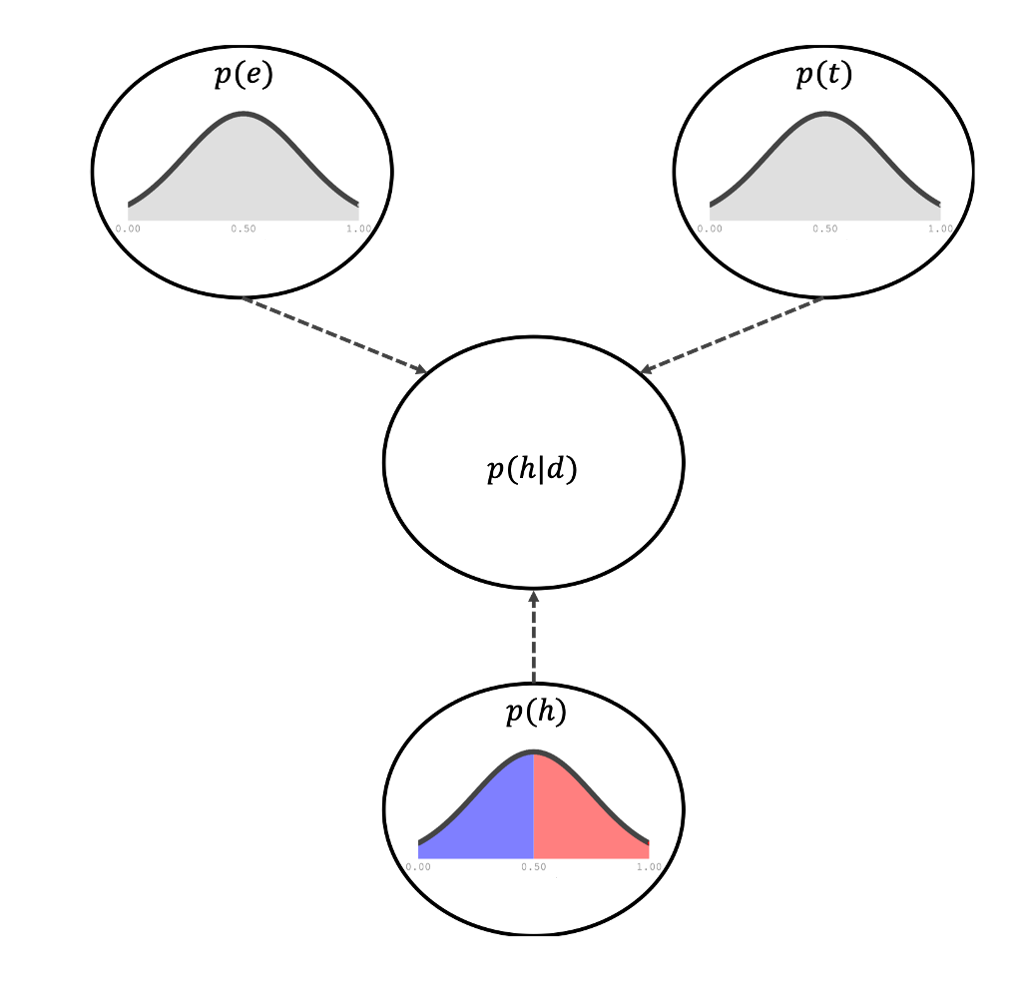
\includegraphics[width=1\columnwidth]{img/bscm_update_2.png}
\caption{Figure shows how a prior belief and the perceived credibility of a source (operationalized via expertise and trustworthiness) interact within the BSCM framework. For the present simulations, agents sampled \(P(h)\), and subjective \(e\) and \(t\) estimates from univariate Gaussian distributions (\(\mu\) = 0.50, \(\sigma^2\) = 0.20). Values between 0.00 and 0.50 (blue) =  \(P(\neg h)\); Values between 0.51 and 1.00 (red) =  \(P(h)\). Distributions were truncated (range: [0, 1]).} 
\label{fig:rich_vis}
\end{figure}


In the BSCM framework, the likelihood for an agent that supports a hypothesis  \(P(h)\) is given by

\begin{equation}
    P(d|h) = \sum_{e't'}P(h|e',t')P(e')P(t'). 
\end{equation}

In the same way, the likelihood for an agent that does not support a hypothesis \(P(\neg h)\) corresponds to
   
\begin{equation}
    P(d|\neg h) = \sum_{e't'}P(\neg h|e',t')P(e')P(t') 
\end{equation}

(see \cite{hahn2009argument, harris2016appeal}, for further details).   Table 1 shows the   conditional probability table which specified how the different components of the likelihood were computed. Here, expertise strength, \(\textbf{\emph{e}}\), determines how strongly a communication target is influenced by the expertise of a source (robustness check 1). Conceptually, expertise strength can be thought of epistemic authority (i.e., knowledge superiority; see also \cite{walton1997pennsylvania, harris2016appeal}), which suggests that a source with higher expertise strength is going to exert stronger influence on a receiver during belief formation.

To explore the impact of knowledge superiority, we investigated the influence of three different parameter settings for expertise strength on echo chamber formation (see Table 2). To ensure that the direction of the influence of expertise strength matched an agent's prior belief (i.e., towards 1 if \(P(h)\) > 0.5 and towards 0 if  \(P(h)\) < 0.5), we flipped the impact of expertise strength based on the prior. Similar to an indicator function, \(\textbf{\emph{I}}\) thus returned 1 for agents having a prior belief \(P(h)\) > 0.5 and -1 for agents having a prior belief \(P(h)\) < 0.5.\footnote{\(\tau\) is an additional constant that quantifies the presence vs. absence of expertise (\(\tau\) = 2 for all simulations).}

\begin{table}[!h]
\footnotesize
\begin{center} 
\caption{Conditional probability table} 
\label{sample-table} 
\vskip 0.10in
\begin{tabular}{c c c c c } 
\hline
 & e,t & \neg e,t & e,\neg t & \neg e,\neg t\\
\hline
h  & \[0.5 + eI_{P(h)>0.5}*\tau \] & \[0.5 + eI_{P(h)>0.5} \] & \[0.5 - eI_{P(h)>0.5}*\tau \] & \[0.5 - eI_{P(h)>0.5}\]\\
\neg h & 1 - (0.5 + eI_{P(h)>0.5}*\tau) & 1 - (0.5 + eI_{P(h)>0.5}) & 1 - (0.5 - eI_{P(h)>0.5}*\tau) & 1 - (0.5 - eI_{P(h)>0.5})\\
\hline
\end{tabular} 
\end{center} 
\end{table}

\subsubsection{Social and asocial agents}
The BSCM architecture provides a general framework for updating one's belief under consideration of a source's credibility. It does not specify how individual agents estimate the perceived expertise and perceived trustworthiness values of a source during interaction. Here, we assume that social media users take the beliefs of their peers into consideration when evaluating the credibility of a source. Based on this assumption, each agent in our first population of social agents is furnished with subjective estimates of \(e\) and \(t\) sampled from univariate Gaussians (see Fig. 1). Following observation of a source's belief in a hypothesis, the target agent (receiver) then evaluates the perceived expertise and trustworthiness of the communicating source. Based on our assumption that beliefs of network peers matter during the evaluation of a source's credibility, a receiver then computes  weighted  for the source. These weighted \(P(e)\) and \(P(t)\) based on the proportion of agents in the receiver's direct network entertaining the same belief as the source and the number of agents in the network entertaining the opposite belief of the source. Additionally, the perceived expertise and trustworthiness values are weighted by the individual \(e\) and \(t\) of agents in the receiver's direct network. More formally, this can be written as  

\begin{equation}
    P(e) = \frac{\sum_{i=1}^{N_h}e_i}{\sum_{i=1}^{N_h}e_i + \sum_{i=1}^{N_{\neg h}}e_i}              
\end{equation}

\begin{equation}
    P(t) = \frac{\sum_{i=1}^{N_h}t_i}{\sum_{i=1}^{N_h}t_i + \sum_{i=1}^{N_{\neg h}}t_i}.
\end{equation}

% (which is a function of the weighted proportion of agents supporting the same belief as the source compared to the total number of believers in a receiver's network).

We contrasted the above population of social agents with a second population of asocial agents which randomly sampled perceived expertise and perceived trustworthiness of a source from a uniform distribution bounded between [0, 1]. Asocial agents were used to test the relevance of our assumptions that social media users consider the beliefs of their peers during the credibility estimation of a source. To ensure this, asocial agents sampled stochastic credibility estimates for a source irrespective of the beliefs of their direct network peers. In both populations (social and asocial), the perceived expertise \(P(e)\) and trustworthiness \(P(t)\) estimates were plugged into Equations 2-3 to compute the likelihood of observing a source's belief given the receivers prior belief and the credibility of the source.

\section{Simulations}
Agents were randomly assigned to x-y coordinates in a 2-dimensional space forming links with their nearest neighbors (refer to \cite{wilensky2015introduction, macal2005tutorial}, for further details on how to spatially allocate agents in ABMs). Proximity was measured in terms of Euclidean distance, which has been used as a proxy for relational proximity in social networks \citep{duggins2017}. Prior to the start of a simulation, each agent sampled their own prior belief \(P(h)\) and subjective \(e\), and \(t\) values from a univariate Gaussian with \(\mu\)=0.5 and \(\sigma^2\)=0.20 (for all three estimates). Thus, \(P(h)\), \(e\), and \(t\) differed heterogeneously within our agent population. Following revision of their prior belief according to BSCM, agents declared for one of the two beliefs based on a deterministic decision rule\footnote{If \(P(h)\) = 0.50, an agent declared either belief with a probability of 50\%.}: 

\[
Belief = \begin{cases}
h \text{ if } P(h|d) > 0.5 \\
\neg h \text{ if } P(h|d) < 0.5 
\end{cases}
\]

The declared belief (i.e. \(h\) or \(\neg h\))  was then made pubic based on the P(Declaration) probability (robustnes check 2) which was manipulated between simulations (see Table 2). For example, a declaration of 1 means all agents made their beliefs public, while 0.1 means that there is a 10\% probability for each agent making their opinion public. The conceptual motivation for P(Declaration) is based on recent findings showing that \emph{most} social media users do not discuss their political beliefs on social media, but mainly focus on exchanging shared hobbies and passions \citep{newman2019reuters}. We wanted to ensure that our simulation results are robust across social networks varying in terms of the percentage of users discussing their beliefs with their peers. We thus explored the formation of echo chambers across three levels of P(Declaration) which can be thought of as a proxy for the percentage of people exchanging their beliefs about a particular topic (e.g., politics or news). 

In addition to P(Declaration), we varied the connectivity density between simulations (number of links per agent / total number of agents in the network) from 0.5\% to 50\% (robustness check 3). This allowed us to check whether the formation of echo chambers would change as a function of the number of links each agent has as compared to the total number of agents. Here, more links can be thought of as increased access to information (i.e., knowing about the beliefs of more users). This can be compared to an increased number of friends on Facebook or followers on Twitter, where the information load of a user's News Feed increases if the person has more friends (Facebook) or follows more users (Twitter). 

Simulations were initiated through a neutral event node placed in the center of the simulation (i.e. central x-y-coordinate). Neutral in this case means that the first agent sampled randomly from the set of beliefs \{\(h\), \(\neg h\)\} each time it communicated to a target. Due to this stochastic process, on average, half of the \(1\textsuperscript{st}\) generation agents receiving input from the neutral event node should arrive at belief \(h\) while the other half will arrive at belief \(\neg h\) after BSCM integration. The number of agents the neutral event node communicated to was determined by the connectivity density. Connectivity values above 50\% were omitted as this would have enabled every other agent to be connected to the neutral event node in the 1st generation, precluding the occurrence of a cascade. Similarly, values below 0.5\% would have resulted in fracturing of the network (thus preventing the occurrence of cascades).

\begin{table}[!h]
\footnotesize
\begin{center} 
\caption{Manipulated variables.} 
\label{sample-table} 
\vskip 0.10in
\begin{tabular}{c c c} 
\hline
Name & Description & Levels\\
\hline
Connectivity density (\%) & (Links per Agent / Total Number of Agents) * 100 & 0.5, 1.0, 1.5, ... 50.0\\
Expertise strength & Manipulate the magnitude of expertise influence & 0.00, 0.10, 0.20\\
P(Declaration) & Probability of making a belief public & 0.10, 0.50, 1.00\\
\hline
\end{tabular} 
\end{center} 
\end{table}

After revising their prior beliefs following the equations outlined in the BSCM section, the first-generation agents (those that received input from the neutral event node) made their beliefs public based on the manipulated P(Declaration) value. Their linked neighbours (i.e., second-generation) then used the communicated opinion of the first-generation agents as input for their own belief revision following the same procedure. Thereafter, the process of transmitting beliefs continued down successive generations until the network was either completely saturated (i.e., all agents committed to a belief) or the number of believers (i.e., \(h\) or \(\neg h\)) did not change for two consecutive time periods. As one aim of the present work was to show that a single pass-through of information (i.e., single interaction) is sufficient for the formation of echo chambers, we did not allow for repeated interaction, meaning that agents were no longer attentive to further information once they declared a belief.

To measure echo chambers effectively across simulations, we were first interested in measuring global proportions of beliefs across the whole network (i.e. the relative number of agents with belief \(h\) compared to agents entertaining belief \(\neg h\)). Based on previous simulation based work, we expected that global would consistently approximate 50/50 across both agent populations \citep{pilditch2017opinion}. This measure was necessary to ensure that echo chambers are not a by-product of a dominant network-wide belief. 

Following checks for possible network-wide belief confounds, our key dependent measure of echo chamber formation was the average percentage of like-minded neighbours an agent possessed (i.e., the \textit{local} network similarity). This measure corresponded to the average percentage of agents in the target's direct network that shared the same belief as the target. For example, 50\% means that, on average, agents had equal proportions for each belief type in their direct network, where direct network refers to the fraction of the whole network that is directly connected to a user. Following previous work \citep{pilditch2017opinion}, we expected that social agents would show increased percentages of like-minded neighbours (i.e. echo chambers) for low connectivity density values. We did not expect clustering effects in the asocial population in which agents computed stochastic credibility estimates for a communicating source.

Each system specification was ran (connectivity density (100) x expertise (3) x P(Declaration) (3)) independently 50 times, taking an average set of values for each specification. The total number of agents (n = 1000) was consistent across simulations. Simulations were conducted independently for each of the two agent populations.

\section{Results}
Fig. 2 summarizes our central findings. We predicted that for both social and asocial agents, global belief proportions would consistently approximate 50/50. Fig. 2A (social agent population) and Fig. 2B (asocial agent population) confirm these predictions. Specifically, Fig. 2A and 2B show that global proportions of beliefs in both populations consistently approximated 50/50 irrespective of varying P(Declaration), connectivity density, or expertise strength. This finding is important, as it ensures that potential clusters of like-minded others (Fig. 2C-D) do not result from a global bias towards either belief.

For social agents, the average proportion of like-minded neighbors (Fig. 2C) increased as a function of increasing expertise strength, increasing P(Declaration) and decreasing connectivity density (x-axis). Importantly, to fully reduce the formation of echo chambers, the average network member must be connected to around 15-20\% of the network, which is infeasible considering the size of real world social networks which can have several Billion users. These results are comparable to previous simulation-based work exploring echo chamber formation in a a population of stochastic reinforcement learners \citep{pilditch2017opinion}, although the present findings show less intense clustering effects.

Fig. 2D shows the results from our asocial agent population. As seen in Fig. 2D, if agents were agnostic of their social network, meaning that they stochastically sampled credibility estimates for each source, no echo chambers emerged. This finding highlights the importance of our assumption that users consider the beliefs of their peers during the evaluation of a source's credibility, and it is the main limitation of our findings. The finding in the left panel of Fig. 2D(P(Declaration) = 10\%) showing a reduced clustering effect for connectivity density values below 5\% is of no further relevance as it can be fully attributed to fracturing of the network (i.e., no information cascade occurred). To visualise the above findings, Fig. 3 includes example outcomes of post-cascade belief proportions with 1\% and 5\% connectivity density. A and C correspond to our asocial agent population and B and D pertain to the asocial population. 


\begin{figure}[!t]
\centering
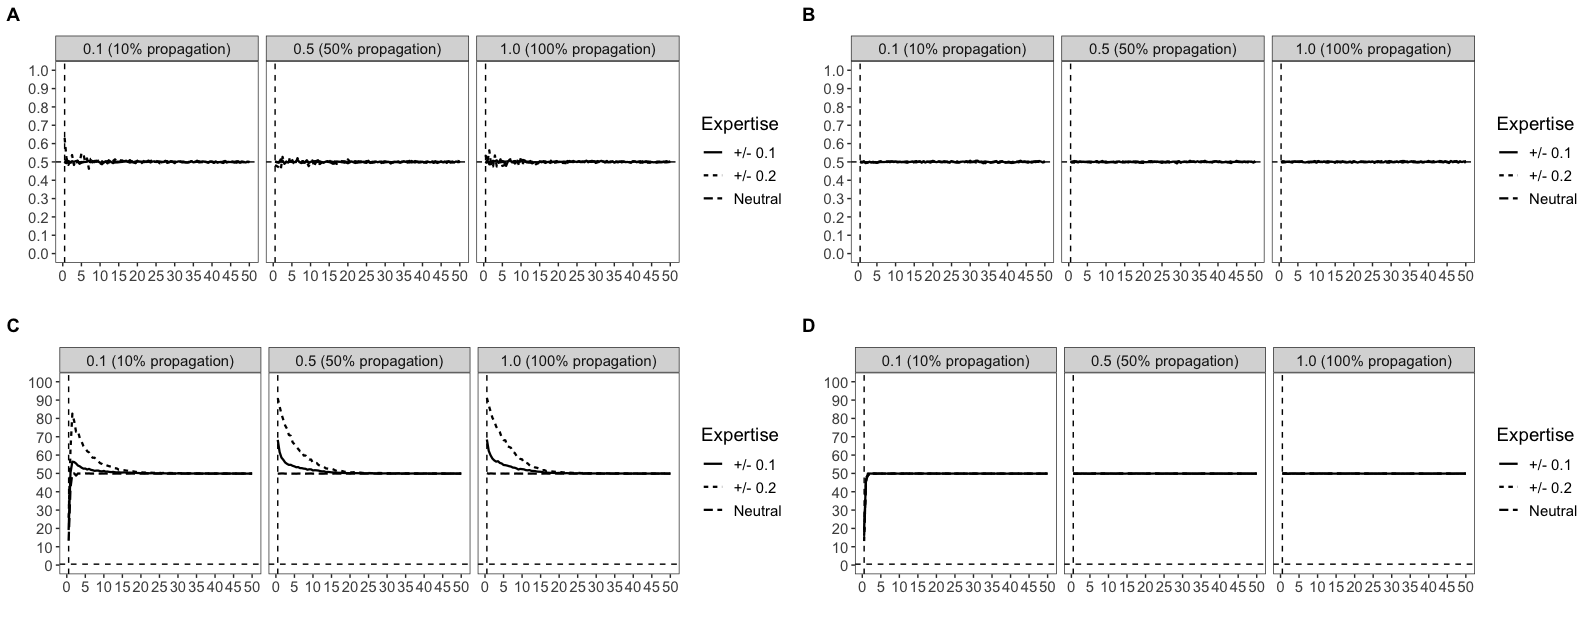
\includegraphics[width=1\columnwidth]{img/results.png}
\caption{Main results. A: global belief proportions, social agents. B: global belief proportions, asocial agents. C: average percentage of like-minded neighbors (i.e. echo chambers), social agents. D: average percentage of like-minded neighbors (i.e. echo chambers), asocial agents.} 
\label{fig:rich_vis}
\end{figure}


\begin{figure}[!t]
\centering
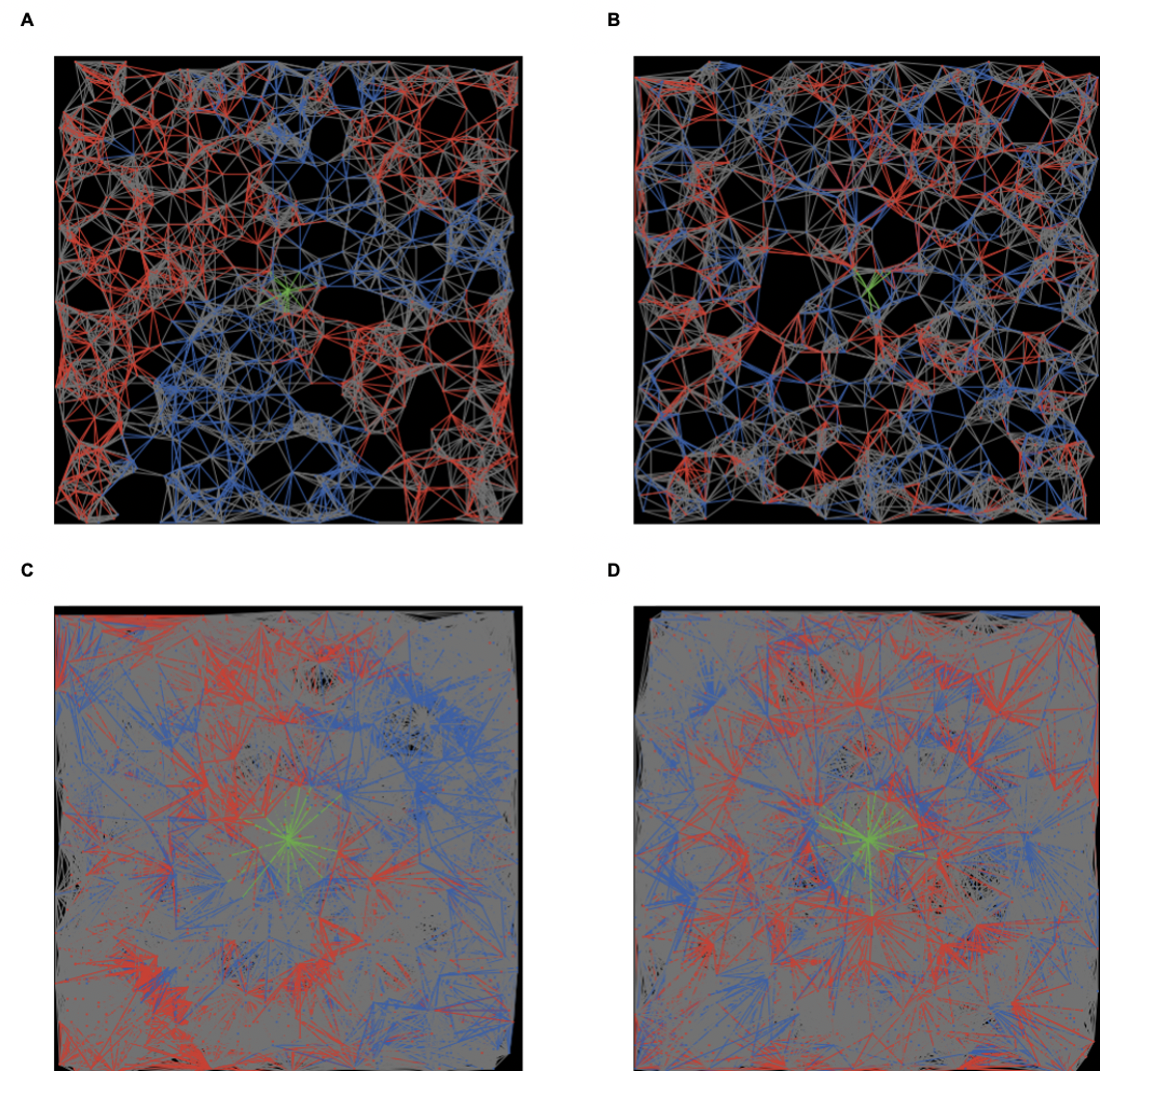
\includegraphics[width=1\columnwidth]{img/example_networks.png}
\caption{Example post-cascade networks. Grey = agents that did not declare a belief; blue = agents believing \(\neg h\); red = agents believing \(h\). Connectivity density values of upper networks: A (social agents): 1\%; B (asocial agents): 1\%. Connectivity density values of lower networks: C (social agents): 5\%; D (asocial agents): 5\%.} 
\label{fig:rich_vis}
\end{figure}


\section{Discussion}
The aim of this work was to disentangle previously conflated causes of echo chambers on social media. Specifically, we examined whether echo chambers emerge in a population of homogeneous, individually rational users that engage in a single interaction. Under the assumption that users evaluate the credibility of a communicating source based on the beliefs of their peers, our results from the social agent population show that echo chambers emerge in a population of individually rational agents who integrate the beliefs of others with their own prior beliefs in a Bayesian manner. Moreover, we showed that echo chambers emerge through a single pass-through of information prior to repeated interaction.

These results suggest that previously identified causes of echo chambers, including psychological biases and inter-individual differences in terms of the cognitive architecture of agents, might not be necessary for the observation of echo chambers. Furthermore, our findings suggest that repeated interaction, which has been a key component in previous models of echo chambers \citep{madsen2017growing, madsen2018large}, might not be required for the formation of echo chambers. On average, each belief was equally represented in our simulations. Thus, our results further show that segregated groups did not evolve as a consequence of a global dominance of a particular belief (see Figs. 2-3). 

Overall, our findings illustrate that echo chambers, which might induce spreading and retention of misinformation, conspiratorial thinking, and political polarization, are not necessarily caused by the inhabitants of social networks directly. Rather, the \textit{structure} of social networks, and notably the constraining lateral (i.e., peer-to-peer) transmission of information can be sufficient for echo chamber formation. The degree of making opinions public (P(Declaration)) did affect echo chamber formation only if it was so low that it effectively fractured the functional message passing around the network. Additionally, the magnitude of expertise strength modulated the influence of credibility, resulting in increased echo chamber effects for higher levels of expertise. This suggests that selecting one's network peers based on epistemic authority (i.e., knowledgeability of other users) might exacerbate the formation of echo chambers. Given that the present simulations included rational Bayesian agents, it is further expected that incorporation of additional psychological variables, such as confirmation bias \citep{del2016spreading, ngampruetikorn2016bias}, might intensify the strength and persistence of echo chambers (see also \cite{pilditch2017opinion}).

More generally, our results show that agent-based models, which enable capturing of dynamic interactions between individuals, provide a valuable opportunity for studying the formation of emergent phenomena such as echo chambers. This is in line with a growing body of literature employing agent-based models to investigate several related phenomena, including opinion polarization \citep{duggins2017}, identity search \citep{watts2002identity}, disbelief in climate change \citep{lewandowsky2019influence} and micro-targeting \citep{madsen2018method}. Given the potential of agent-based models for studying echo chambers and related emergent phenomena, it is important that further work develops interventions which might reduce the occurrence of opinion segregation. Such interventions might extend previous work suggesting that ''educational broadcasts'' across a network of idealized Bayesian agents (similar to the present model) reduce echo chamber formation \citep{madsen2018large}.

The main limitation of our work is the fact that our findings only applied to the social agent population. This finding is central to our paper, as it shows that consideration of the beliefs of network peers while revising one's own beliefs is essential for the observation of echo chambers. If agents sampled stochastic credibility values for communicating sources (asocial population), the network did not show any signs of echo chambers. Further empirical work should thus focus on the validity of this assumption and test whether people down- or up-weigh the credibility of someone that agrees/disagrees with their peers. 

An additional avenue for further work might be a closer examination of the belief updating process of the present agent populations. Specifically, agents in the present populations updated beliefs sequentially based on the declarations of previous generations. Related theoretical work on information cascades has illustrated that sequential updating processes, where people learn from the beliefs and behaviours of others, can result in erroneous collective outcomes \citep{bikhchandani1992theory}. Critically, this work has shown that erroneous collective behaviours emerged regardless of the fact that people integrated beliefs of others in individually rational ways. 

However, recent empirical studies demonstrated that people are sensitive to statistical dependencies in social learning. Specifically, across both abstract (e.g., estimating the number marbles in an urn; see \citet{whalen2018sensitivity}) and more applied tasks (e.g., rating the suitability of a political candidate for public office), it has been shown that people differentiate between the evidential signal of independent beliefs and dependent beliefs that were formed sequentially. As a result, given that the beliefs of others were formed sequentially, people updated their prior beliefs to a smaller extent. \cite{whalen2018sensitivity} interpreted this finding as a potential way of counteracting the formation of information cascades, which have been shown to induce convergence towards like-minded clusters \citep{bikhchandani1998learning}. Given these findings, an important step for future research involves testing the robustness of echo chambers between varying levels of belief dependencies in a network. Here, empirical findings by \citep{whalen2018sensitivity} and (...) might be used as input validation for simulation, enabling agents to differentiate between independent and sequentially updated beliefs. 

In summary, while the study of echo chambers does by no means exhaustively addresses the issue of digital misinformation, it provides an important contribution to our understanding of how people settle on beliefs in social networks. Here, we showed that echo chambers emerge as a consequence of social network structure, including limited access to information (i.e., local connectivity) and lateral transmission of information between social agents. This suggests that social networks themselves can be argued to be causally sufficient for echo chamber formation, while previously conflated causes such as psychological biases, inter-individual differences, and repeated interaction, might not be necessary. Rather, such inter-individual differences and psychological variables, including confirmation bias, are expected to exacerbate the formation of echo chambers \citep{pilditch2017opinion}. Finally, by showing that the computations involved in evaluating the credibility of a source play a key role in the formation of echo chambers, our findings might provide important insights for improving the architecture of social networks in a way to be more robust towards echo chamber formation.


\section{Methods}

\subsubsection{Agent-based Simulations}
The presented agent-based model was implemented in NetLogo version 6.0.4 \citep{wilensky1999netlogo}. All simulations were performed in R using the package {\tt RNetLogo()} \citep{thiele2014r}. The full model including all technical details has been uploaded to Github and can be found via \href{}{ link}. Here we outline the three basic steps involved in our model. 

Algorithm 1 shows the setup procedure of the network.


\begin{algorithm}[H]
\caption{Setup Network}\label{setup}
\begin{algorithmic}[1]
  \Procedure{Place agents}{}
    \State Create $N$ agents
    \For{$i=1$ to $N$}
        \State set i position random x-y coordinate
     \EndFor
  \EndProcedure
  \Procedure{Setup priors and Links}{}
    \For{$i=1$ to $N$}
      \State $P(h)[i]\gets x$\thicksim$N(\mu, \sigma^2)$ 
      \State $P(e)[i]\gets x$\thicksim$N(\mu, \sigma^2)$
      \State $P(t)[i]\gets x$\thicksim$N(\mu, \sigma^2)$
      \State create links with $n$ nearest neighbors \Comment{based on Euclidean distance}
     \EndFor
  \EndProcedure
\end{algorithmic}
\end{algorithm}

Algorithm 2 shows the basic steps involved in a single instance of belief updating (i.e., from one generation to the the next). Here, source refers to an agent from the previous generation that already publicly declared a belief (i.e., \(h\) or \(\neg h\)).

\begin{algorithm}[H]
\caption{Updating beliefs}\label{update}
\begin{algorithmic}[1]
  \Procedure{Source selects communication target}{}
    \If{matchCounter $\leq$ 1}
        \For{$i=1$ to $n_{source}$}\Comment{n = source's connections}
            \If{i = neutral}\Comment{check if agent did not already declare a belief}
             \State belief[i] = BSCM(source, n[i])\Comment{n = target's connections}
              \If{random(0.01,1.00) > P(Declaration)}
               \State propagate belief to next generation
              \EndIf
             \EndIf
        \EndFor
    \EndIf
  \EndProcedure
\end{algorithmic}
\end{algorithm}

Algorithm 3 illustrates how the {\tt matchCounter} variable shown above was updated. If there was no change in overall proportions of beliefs for two consecutive time periods (i.e., the network was either saturated or fractured), simulations stopped.

\begin{algorithm}[H]
\caption{Proceed to next generation}\label{proceed}
\begin{algorithmic}[1]
  \Procedure{Check if network is saturated or fractured}{}
    \State matchCounter = 0 \Comment{counts how often no change occurred between generations}
    \State Count_{\(h\)} = 0
    \State Count_{\(\neg h\)} = 0
    \For{$i=1$ to $N$}\Comment{N = all agents}
        \If{belief[i] = \(h\)}
            \State Count_{\(h\)} = Count_{\(h\)} + 1
        \EndIf
        \If{belief[i] = \(\neg h\)}
            \State Count_{\(\neg h\)} = Count_{\(\ \)} + 1
        \EndIf
    \EndFor
    \If{Count_{\(h\)} = Count_{\(\neg h\)}}
        \State matchCounter = matchCounter + 1
    \EndIf
  \EndProcedure
\end{algorithmic}
\end{algorithm}

\newpage

\bibliographystyle{apacite}
\bibliography{refs}


\end{document}